\chapter{Другий клас}

\problem
Діти збирали горіхи. Маша в~кошик поклала 17~горіхів.
Федько~--- на 12 більше, ніж Маша. А~Іванка~--- на 14 менше, ніж Федько.
Скільки горіхів разом зібрали діти?


\problem
У~Іванки в~зошиті лишилося 8~чистих аркушів.
У~Марії~--- на 6~аркушів менше.
А~у~Федька стільки, скільки у~дівчат разом.
Скільки чистих аркушів лишилося в~зошиті кожного з учнів БеркоШко?


\problem
Міша і~Сергій привезли з~базару 5~кг картоплі, 2~кг моркви,
3~кг цибулі й~1~кг буряків.
Прибігли школярики і допомогли принести до школи 6~кг овочів.
Які овочі принесли діти до школи?


\problem
\problemname{Дослідження циферблату}

\begin{figure}[h]
    \centering
    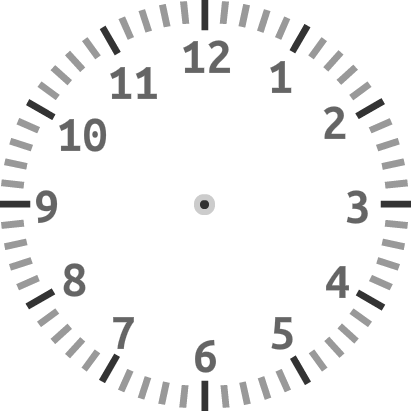
\includegraphics[width=0.3\textwidth]{2-04-1}
\end{figure}

Якщо годинна стрілка стоїть на~2, де вона опиниться через 3~години?
Якщо стоїть на~10, де буде через 5~годин?
На~11, де буде через 18?


\problem
Запиши математичною мовою словесні вирази:
\begin{enumerate}
    \item Число 7 збільшили на~12.
    \item 24 зменшили на~8
    \item Різниця між числами 5 і~8.
    \item Від 15 забрали 3.
    \item 13 додали до 3.
    \item Сума чисел 7 і~4.
    \item Взяли разом 3 і~5, а~потім додали до суми чисел 7 і~4.
    \item Від різниці чисел 10 і~4 мають забрати різницю чисел 5 і~3
\end{enumerate}
Яка відповідь вийде у~кожному з~випадків? Обчисли.


\problem
Роздивися математичний вираз:
\[
(4 - 2) + 5 + (7 - 3) - (10 - 3)
\]
\begin{enumerate}
    \item Скільки арифметичних дій (додавань та віднімань)
    треба зробити, щоб отримати відповідь?
    \item Виконай дії у~правильному порядку.
    Окремо запиши кожну дію, що виконав.
    \item Спробуй прочитати та записати цей вираз словами
    (подібно до того, як записані словесні вирази в~попередньому завданні).
\end{enumerate}


\problem
В~понеділок Сашко не встиг придумати 16~завдань з~математики,
з~них 6~--- для Федька, а~решту~--- для Марії та~Іванки порівну.
У~вівторок Сашко не встиг придумати ще 5~завдань,
по~2 для Іванки з~Федьком, а~решту~--- для Марії.
Коли прийшла середа, Сашко захотів придумати
ще по~2 завдання для кожного з~учнів, але знову не встиг.
А~потім настав четвер, у~БеркоШко почалися заняття
і~придумувати завдання з~математики було вже запізно.

Питання:
Скільки всього завдань з~математики не встиг придумати Сашко цього тижня?
Для кого з~учнів Сашко не встиг придумати найбільше завдань?
Чи відрізняється кількість непридуманих завдань для кожної з~дівчат?
Якщо так, то на скільки?
Для кого Сашко не встиг придумати парну, а~для кого непарну кількість завдань?


\problem
Обідали 8~вовченят і~6~зайченят. Було 10~морквин і~8~котлет.
Відомо, що кожна тваринка з'їла те, що їй зазвичай подобається
і~рівно по одній.
Скільки котлет залишилося? А~морквин? Запиши розв'язок охайно.


\problem
Маша стрибнула в~довжину на 1~метр.
Федьковий результат відрізняється на 23~сантиметри.
На яку відстань стрибнув Федько?


\problem
Знайди і~виправ помилки:
\begin{multicols}{2}
    \begin{enumerate}
        \item $37 + 12 = 50$
        \item $27 - (9 + 3) = 15$
        \item $32 - (11 - 7) = 28$
        \item $11 + 11 + 11 = 44$
        \item $(16 - 8) + 13 = 22$
        \item $(13 + 8) - (13 - 8) = 16$
        \item $(13 + 8) + (13 - 8) = 16$
        \item $(13 - 8) + (13 - 8) = 13$
    \end{enumerate}
\end{multicols}


\problem
Накресли один відрізок довжиною у~стільки сантиметрів, скільки тобі років.
А~другий відрізок~--- скільки років твоєму молодшому братикові чи сестричці.
За малюнком визнач, на скільки років ти старший.
Запиши розв’язання прикладом.


\problem
Зранку Марія принесла до БеркоШко новорічний подарунок у~червоній коробці.
Всередині було 42~цукерки.
Весь день діти вчились, грались, обідали і~поїли всі цукерки.
Впродовж дня Марія з’їла 12~цукерок, Федько~--- на~2 більше, ніж Марія,
а~Іванка~--- на~4 менше, ніж Федько.
Пригостили також і~меншеньких. Платонові й~Василькові дісталося по 2~цукерки.
А~Варуся одну цукерку з’їла сама, а~іншу~--- віддала Іванці.

Хто в~БеркоШко з’їв більше цукерок: хлопчики чи дівчатка?
Запиши скорочену умову, зроби малюнок, запиши розв’язок
математичною мовою (прикладами) і~відповідь.


\problem
Виріши приклади, запиши проміжну дію:
\begin{multicols}{2}
    \begin{enumerate}
        \item $(22 + 7) - (21 - 13) =$
        \item $(22 - 7) + (21 - 13) =$
        \item $(22 - 7) - (21 + 13) =$
        \item $(22 + 7) + (21 - 13) =$
        \item $(22 - 7) + (21 + 13) =$
        \item $(22 + 7) - (21 + 13) =$
        \item $(22 - 7) - (21 - 13) =$
        \item $(22 + 7) + (21 + 13) =$
    \end{enumerate}
\end{multicols}


\problem
Татусі вирішили зробити дітям гойдалку в~дворі висотою 1~м і~80~см.
Привезли два стовпи-опори довжиною 2~м 40~см.
Якої глибини мають бути ями, щоб вкопати опори для гойдалки?


\problem
Суботнім ранком у~дворі БеркоШко мужики рубали дрова.
Спершу Сергій розрубав 3~колоди, кожну на 4~полінця.
Потім Сашко розрубав ще 4~колоди, кожну також на 4~полінця.
А~Андрій рубав колоди лише навпіл, розрубав 8~колод.
Потім вони зібрали усі полінця і~склали під лежанкою біля пічки.

Скільки полінець лежить під лежанкою?
Запиши скорочену умову, зроби малюнок,
запиши розв’язок математичною мовою (прикладами) і~відповідь.


\problem
Де трикутників більше?

\begin{figure}[h]
    \centering
    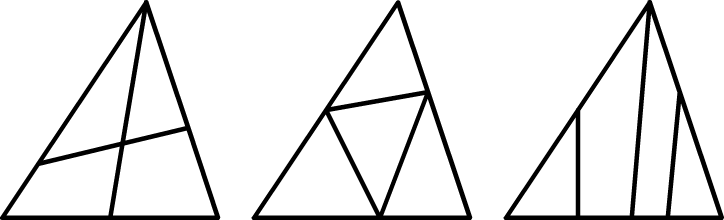
\includegraphics[width=0.6\textwidth]{2-16-1}
\end{figure}


\problem
У~Василька було трохи копійочок.
Якось він знайшов монетку в~10~копійок, а~потім ще п’ятачок.
Він попросив Федька порахувати, скільки в~нього тепер стало грошей,
виявилося, що 59~копійок.
Скільки копійок було у~Василька спочатку?
А~які монетки могли в~нього бути? 


\problem
Аркуш із завданнями забули на столі і~малята заляпали його фарбою так,
що деякі цифри зовсім пропали.
Але ми все-таки спробуємо їх розв’язати.

Порівняй:
% TODO: 50? why answer everywhere is 50?
\begin{multicols}{2}
    \begin{enumerate}
        \item $25 + 5\hiddendigit \ \square \ 50$
        \item $7\hiddendigit - 11 \ \square \ 50$
        \item $65 + \hiddendigit\hiddendigit \ \square \ 50$
        \item $44 - \hiddendigit \ \square \ 50$
        \item $72 + \hiddendigit\hiddendigit \ \square \ 50$
        \item $28 + 1\hiddendigit \ \square \ 50$
        \item $21 - \hiddendigit \ \square \ 50$
        \item $66 - 3\hiddendigit \ \square \ 50$
    \end{enumerate}
\end{multicols}


\problem
Андрій стрибає в довжину з~місця на 1~м 90~см.
А~хотів би стрибнути на 2~м 60~см.
Наскільки далі потрібно навчитися стрибати Андрієві?


\problem
Знайди якомога більше розгорток кубика на рисунку~\ref{fig:cubes}.

\begin{figure}[h]
    \centering
    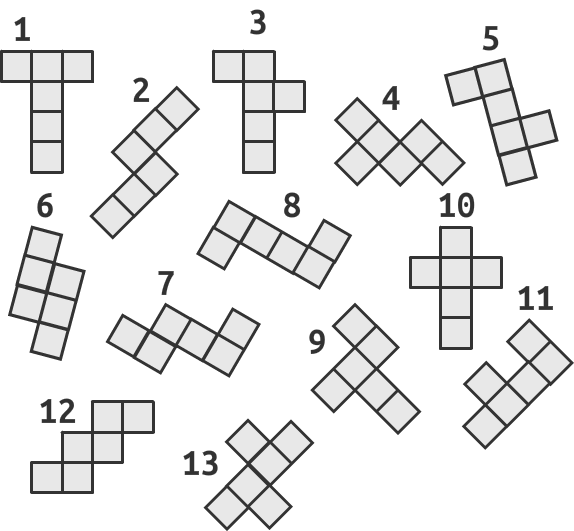
\includegraphics[width=0.6\textwidth]{2-20-1}
    \caption{Можливі розгортки кубика.}
    \label{fig:cubes}
\end{figure}


\problem
На обід у~БеркоШко насмажили 32~котлетки.
Марія, Федько, Іванка, Оля, Катя, Олеся і~Валя з’їли по 2~котлети,
а~Василько, Платон і~Варуся~--- по~1.
На скільки менше котлет залишилось, ніж з’їли за обідом?


\problem
Скільки тобі років?
А~скільки років твоєму братикові чи сестричці?
Скільки років буде тобі, коли твій братик/сестричка стане такий, як ти?


\problem
Яке число знаходиться посередині між:
\begin{multicols}{3}
    \begin{enumerate}
        \item 3 і 5
        \item 7 і 12
        \item 8 і 14
    \end{enumerate}
\end{multicols}


\problem
Скільки горіхів та на яку шальку треба покласти (або забрати),
щоб врівноважити терези, якщо:
\begin{itemize}
    \item на лівій шальці 19~горіхів, на правій~--- 13?
    \item на лівій 12, на правій~--- 24?
    \item на лівій 8, на правій~--- 27?
\end{itemize}


\problem
Ділення:
\begin{enumerate}
    \item 20~яблук розділи між 4~людьми.
    \item 23~олівці розподіли між 3~людьми.
    \item З~16~клітинок склади 4~однакових квадрата.
    \item 9~кошенят треба роздати 4~хлопчикам.
    \item На тарілці було 27~млинців. 5~учнів з'їли майже всі,
    кожен з'їв однакову кількість.
    Скільки млинців з'їли, скільки залишилось?
    \item У~відрі було 34~стакани компоту.
    За день 6~людей випили майже весь компот,
    кожен випив однакову кількість стаканів компоту.
    \item Склади найбільший прямокутник, використавши
    не~більше 23~клітинок.
    \item Склади найбільший прямокутник, використавши
    не~більше 26~клітинок.
    \item На розв'язання кожного прикладу хлопчик витрачає 7~хвилин.
    Скільки прикладів він зможе розв'язати за годину?
    Скільки часу в~нього залишиться?
\end{enumerate}


\problem
Тарган за 3~хвилини проповз 18~метрів.
Він не зупинявся і~повз весь час, не сповільнюючись і не прискорюючись.
Як думаєш, якої довжини шлях він проповзає за 1~хвилину?
А~за 7~хвилин?


\problem
Спробуй намалювати квадрат, що складається рівно з~2~клітинок.
Якщо вийшло, то чи зможеш ти намалювати квадрат,
що складається рівно з~8~клітинок?


\problem
Тато-слон приніс слоненяткові чимало кавунів
і~мама-слониха також трохи принесла.
Слоненя з’їло частину тих кавунів.
Скільки кавунів залишилось?


\problem
У~БеркоШко було 4~дітей. Кожний з’їв по 3~оладки.
А~залишилося вдвічі більше, ніж діти з’їли.
Скільки було оладок?


\problem
У~Робіна Гуда в~колчані було чимало стріл.
Він прийшов на турнір і~стріляв по мішенях.
В~кожну мішень він влучив однакову кількість разів
і~жодного разу не промахнувся.
Після змагання в~нього залишилося трішки стріл.
Як дізнатися, скільки стріл Робіна влучило в~кожну мішень?


\problem
У більшості випадків речення звичайної мови розповідають про людей, об'єкти,
переповідають думки.
Але бувають речення, що розповідають самі про себе.
Наприклад, ці речення розповідають про себе і~кажуть правду:
\begin{itemize}
    \item Це речення написане українською мовою.
    \item Я придумане Сашком і~надіслане до тебе
    за допомогою комп’ютерної мережі.
\end{itemize}
Ще приклад (з~російської мови):
\begin{itemize}
    \item В~этой фразе двадцать восемь букв.
\end{itemize}
А~от приклад речення, що розповідає про себе, але неправду:
\begin{itemize}
    \item Ти не зміг мене прочитати.
\end{itemize}

% TODO: вставити сюди типу "Завдання:"
\begin{enumerate}
    \item Придумай принаймні 8~речень що розповідають про себе.
    Серед них має бути половина правдивих, а~інша половина~--- неправдивих.
    \item Спробуй придумати правдиве речення про кількість букв
    у~самому собі українською мовою. 
    \item Спробуй придумати речення що розповідає саме про себе,
    але не вдається визначити, чи воно правдиве, чи ні.
\end{enumerate}


\problem
В~одній країні стався сильний снігопад~--- за одну ніч
(з~вечора до ранку~--- за 12~годин) випало близько 8~см снігу.
З'ясуй, якщо~б сніг продовжував так само падати і~далі,
то за який час він~би повністю засипав значну частину легкових автомобілів.
(Якщо тобі раптом здалося, що чогось в~умові задачі не~вистачає,
проведи необхідні досліди або вимірювання).


\problem
Які числа можна записати замість букв, щоб рівності стали вірними?
\begin{enumerate}
    \item $(5 + \textit{п}) : 4 = 23$ (і~остача 3)
    \item $25 + (23 - 3 \cdot \textit{к}) \cdot 2 = 47$
\end{enumerate}


\problem
Придумай три приклади, для яких наступне має бути правдою.
\begin{enumerate}
    \item Кожен приклад має складатись з~чотирьох чисел~--- 16, 12, 6, 4,
    поєднаних трьома діями~--- додаванням, відніманням та множенням.
    Якщо потрібно можна використовувати дужки.
    \item В~першому прикладі можна за бажанням або
    спочатку виконати множення або додавання;
    \item В~другому прикладі обов'язково другою дією має
    виконуватися множення (не вийде його виконати першим або останнім);
    \item В~третьому прикладі множення обов'язково має бути останньою дією.
    \item У~всіх трьох прикладах вийде зробити всі обчислення і~отримати відповідь.
\end{enumerate}
Знайди ці відповіді.


\problem
Запиши математичною мовою і~знайди значення виразів:
\begin{enumerate}
    \item різниця чисел 34 і~23;
    \item сума чисел 35 і~27;
    \item різниця чисел 25 і~76;
    \item добуток чисел 3 і~15;
    \item чотири рази по дев'ять;
    \item п'ять десятків і~сім взяли разом із шістьма десятками;
    \item добуток чисел 3 і~4 взяли разом із різницею чисел 7 і~5.
\end{enumerate}


\problem
\problemname{Спостереження за дужками}
У~виразі $10 - 4 + 3 - 2 - 1$ спробували розставити дужки різними способами
і~отримали 9 різних виразів:
\begin{multicols}{2}
    \begin{enumerate}
        \item $(10 - 4) + 3 - 2 - 1$
        \item $10 - (4 + 3) - 2 - 1$
        \item $10 - 4 + (3 - 2) - 1$
        \item $10 - 4 + 3 - (2 - 1)$
        \item $(10 - 4 + 3) - 2 - 1$
        \item $10 - (4 + 3 - 2) - 1$
        \item $10 - 4 + (3 - 2 - 1)$
        \item $(10 - 4 + 3 - 2) - 1$
        \item $10 - (4 + 3 - 2 - 1)$
    \end{enumerate}
\end{multicols}
Виконай дії і~знайди значення кожного з~виразів.
Порівняй отримані відповіді із~значенням початкового виразу,
того, що без дужок.
Виявиться, що від розставлення дужок в~деяких виразах змінилося
значення (відповідь), а~в~деяких~--- залишилося таке саме
як було у~виразі без дужок.
Випиши окремо, на одну сторінку, вирази, де присутність дужок
не~змінила значення, а~на іншу сторінку~--- ті вирази,
де від розставлення дужок відповідь змінилася.
Як думаєш, що спільного в~розташуванні дужок у~виразах,
де відповідь не~змінилася?
А~що спільного в~розташуванні дужок у~виразах на іншій сторінці?
Запиши свої думки-відповіді.


\problem
У~багаторукого Шиви 6~рук і~на кожному пальці~--- каблучка.
Скільки каблучок у~Шиви?


\problem
\problemname{Задача за мотивами гри «Супер фермер»}
Ти маєш 14~кролів, 1~вівцю, 3~поросяти і~3~корови.
Скільки коней і~собак ти можеш виміняти, якщо:
\begin{itemize}
    \item 1~кінь = 2~корови,
    \item 1~корова = 3~свині = великий пес,
    \item 1~свиня = 2~вівці,
    \item 1~вівця = 6~кролів = малий пес.
\end{itemize}
Хто залишиться?


\problem
\problemname{Ширина фігур}
Якої найменшої ширини має бути коридор,
щоб через нього зміг пролізти квадратик?
А~який найширший коридор може квадратик перекрити?
Замалюй. Також замалюй найвужчий і~найширший коридор для кола.


\problem
Яке число можна підставити замість букви, щоб рівність стала вірною?
Будь уважним, можливо, в~деяких прикладах замість букви підходить декілька чисел.
\begin{multicols}{2}
    \begin{enumerate}
        \item $А : 12 = 6$
        \item $12 : А = 6$
        \item $12 : А = 1$
        \item $А : 12 = 1$
        \item $А : А = 1$
        \item $А : А = 6$
        \item $А : А = А$
        \item $А \cdot А = А$
    \end{enumerate}
\end{multicols}
